%template1.tex
%The following LaTeX source file represents the simplest kind of slide presentation; no overlays, no included graphics. Substitute your favorite style for ``pascal''. To create the PDF file template1.pdf, (1) be sure to use the prosper class, then (2) execute the command latex template1.tex, and (3) the command dvipdf template1.dvi.

%%%%%%%%%%%%%%%%%%%%%%%%%%%%%%% template1.tex %%%%%%%%%%%%%%%%%%%%%%%%%%%%%%%%%%%
\documentclass[a4paper,blends,pdf,colorBG,slideColor]{prosper}
% definitions for slides for CSC544
% Lutz Hamel, (c) 2007

\hypersetup{pdfpagemode=FullScreen}

\usepackage{amssymb}
\usepackage{latexsym}
\usepackage{amsmath}
%\usepackage[usenames]{color}
\usepackage{xypic}


\newcommand{\term}[1]{\ensuremath{\mbox{\bf #1}}}
\newcommand{\nonterm}[1]{\ensuremath{\mbox{#1}}}
\newcommand{\ifstmt}[3]{\ensuremath{{\bf if}\; {#1}\;{\bf then}\;{#2}\;{\bf else}\;{#3}\;\term{end}}}
\newcommand{\whilestmt}[2]{\ensuremath{{\bf while}\; {#1}\;{\bf do}\;{#2}\; \term{end}}}
\newcommand{\funcstmt}[3]{\ensuremath{{\bf fun}\; {#1}\; {\bf is}\; {#2} \; {\bf return}\; {#3}}}
\newcommand{\syntaxset}[1]{\ensuremath{\mbox{\bf #1}}}
\newcommand{\orbar}{\;|\;}
\newcommand{\bs}[1]{\begin{slide}{#1}\ptsize{8}}
\newcommand{\es}{\end{slide}}
\newcommand{\co}{\,\colon\;}
\newcommand{\pair}[2]{\ensuremath{\langle {#1}, {#2} \rangle}}
\newcommand{\encode}[1]{\ensuremath{\langle {#1} \rangle}}
\newcommand{\mytab}{\makebox[.15in]{}}
%\newcommand{\abs}[1]{{\mid{#1}\mid}}
\newcommand{\abs}[1]{{|{#1}|}}
\newcommand{\ol}[1]{\overline{#1}}

\newcommand{\qaccept}{\ensuremath{q_{\mbox{\tiny accept}}}}
\newcommand{\qreject}{\ensuremath{q_{\mbox{\tiny reject}}}}
\newcommand{\accept}{{\em accept}}
\newcommand{\reject}{{\em reject}}

\newcommand{\machine}[1]{
	\begin{quote}
	{#1}
	\end{quote}
	}

\newcommand{\fdef}[1]{
	\begin{center}
	\fbox{
	\begin{minipage}{3.5in}
	{\bf Definition:}
	{#1}
	\end{minipage}
	}
	\end{center}
	}

\newcommand{\ftheorem}[1]{
	\begin{center}
	\fbox{
	\begin{minipage}{3.5in}
	{\bf Theorem:}
	{#1}
	\end{minipage}
	}
	\end{center}
	}

\newcommand{\flemma}[1]{
	\begin{center}
	\fbox{
	\begin{minipage}{3.5in}
	{\bf Lemma:}
	{#1}
	\end{minipage}
	}
	\end{center}
	}


\newcommand{\fframe}[1]{
	\begin{center}
	\fbox{
	\begin{minipage}{3.5in}
	{#1}
	\end{minipage}
	}
	\end{center}
	}

\newcommand{\nframe}[1]{
	\begin{center}
	\begin{minipage}{3.5in}
	{#1}
	\end{minipage}
	\end{center}
	}

\begin{document}


\bs{$PSPACE$ Completeness}

\fdef{
A language $Q$ is {\bf $PSPACE$-complete} if it satisfies two conditions:
\begin{enumerate}
\item $Q$ is in $PSPACE$,
\item every $L$ in $PSPACE$ is polynomial time reducible to $Q$.
\end{enumerate}
If $Q$ merely satisfies condition 2 we say that it is {\bf $PSPACE$-hard}.
}

\vspace{.2in}
{\bf NOTE:} We chose polynomial time reduction here because we want the reductions to be ``easy''.
\es

\bs{$PSPACE$ Completeness}
The canonical example of a $PSPACE$-complete problem is a generalization of $SAT$ using
formulas with quantifiers,
\[
\forall x \exists y [ (x \vee y) \wedge ( \overline{x} \wedge \overline{y})]
\]

Then the language
\[
TQBF = \{\langle \phi \rangle | \text{$\phi$ is a true fully quantified Boolean formula}\}.
\]

\es

\bs{$PSPACE$ Completeness}
\small
\ftheorem{
\begin{center}
$TQBF$ is $PSPACE$-complete.
\end{center}
}

{\bf Proof:}  First we show that it is in $PSPACE$.

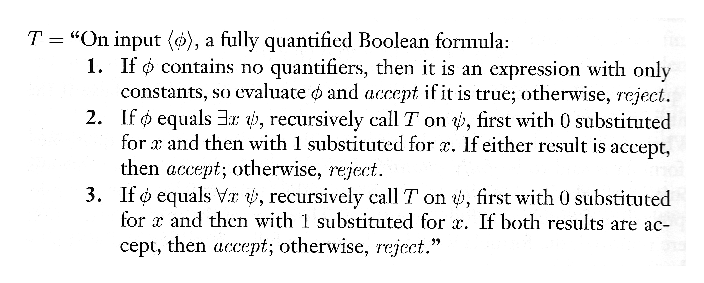
\includegraphics[width=3in]{images/tqbf.eps}

Observe that the machine runs in linear space.

For the second proof obligation it is possible to show that each language $L \in PSPACE$ can
by polynomial time reduced to $TQBF$ by encoding every string in $L$ as a quantified formula.
This is similar to the completeness proof of the $SAT$ problem.
\es

\bs{$L$ and $NL$}
\vspace{.2in}
\fdef{$L$ is the class of languages that are decidable in logarithmic space on a deterministic Turing machine,
\[
L = SPACE(\log n).
\]
$NL$ is the class of languages that are decidable in logarithmic space on a nondeterministic Turing machine,
\[
NL = NSPACE(\log n).
\]
}
\es

\bs{Context-free Languages}
\ftheorem{Let  $A = \{0^k 1^k | k \ge 0\}$, then
\[
A \in L.
\]
}

{\bf Proof:} Observe that a binary counter can store a value $v \le 2^p$  in $\log  2^p = p$ bits.  This allows us to 
build a machine that recognizes this language with two binary counters such that $k \le 2^n$, thus using $O(\log n)$ space.
\es

\bs{$PATH$}
\ftheorem{Let 
\[
PATH = \{ \langle G,s,t\rangle | \text{$G$ is a directed graph with a path from $s$ to $t$}\}
\]
then
\[
PATH \in NL
\]
}
{\bf Proof:} The machine only stores a pointer to the current node and runs a maximum of $m$
iterations where $m$ is the number of nodes.  At each iteration it nondeterministically chooses which
node to visit next.  This machine runs in $\log n$ space where $n = 2^p$ and $p$ is the number of bits required to
count up to $m \le n$.
\es

\bs{Log Space Transducers}

\vspace{.2in}

\fdef{

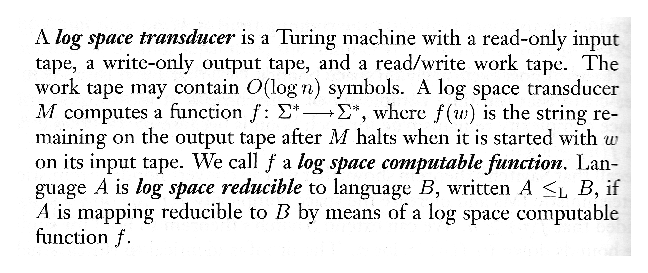
\includegraphics[width=3in]{images/logspace.eps}
}

\vspace{.2in}
\fdef{
A language $Q$ is $NL$-complete if
\begin{enumerate}
\item $Q\in NL$,
\item every $A\in NL$ is log space reducible to $Q$.

\end{enumerate}
}
\es

\bs{$PATH$}
\ftheorem{
\[
PATH \in NL-\text{complete}.
\]
}
(see book for proof.)

Recall that $PATH \in P$, from this and the above it follows that
\[
NL \subseteq P
\]
 (all languages in $NL$ can be reduced to $PATH$ which
in turn is in $P$)
\es

\bs{Putting it all together}

Putting this all together gives us the following hierarchy:
\fframe{
\[
L \subseteq NL \subseteq P \subseteq NP \subseteq PSPACE \subseteq EXPTIME
\]
}
\es

\end{document}
%%%%%%%%%%%%%%%%%%%%%%%%%%% end of template1.tex %%%%%%%%%%%%%%%%%%%%%%%%%%%%%%%%

